\chapter{Coulomb 散射 (Coulomb Scattering)}\label{ch:coulomb}

到目前为止，本书所发展的散射理论 —— 包括第~\ref{ch:Smat1P} 章中
M{\o}ller 算符和 $\Smat$ 矩阵的定义、第~\ref{ch:stationary} 章中
定态散射波函数 $\inn{\vec x}{\vec p+}$ 的渐近形式、第~\ref{ch:partial}
章中相移 $\delta_\ell$ 与分波振幅的引入，以及第~\ref{ch:born} 章中
Born 级数的收敛 —— 都建立在一个核心假设之上：势 $V(r)$ 满足
\emph{短程}条件，例如 $r V(r)\to 0$ 当 $r\to\infty$。这一条件
保证了：自由演化 $\rme^{-\rmi H_0 t/\hbar}$ 能正确地描写在
$t\to\pm\infty$ 时散射粒子的渐近运动；定态波函数具有
``入射平面波 $+$ 球面外向波'' 的标准结构；分波相移 $\delta_\ell$
以及振幅 $f(\theta)$ 都是良定义的。

但是宇宙中最重要、最常见的相互作用之一 —— 两个带电粒子之间的
\emph{Coulomb 相互作用} $V(r)=e_1 e_2/r$ —— \emph{并不}满足上述短程
假设。$1/r$ 衰减得太慢：经典地讲，即使两粒子相距任意远，库仑力
依然在拉拽它们，导致散射轨道永远不能被视为``自由的''；量子地讲，
渐近条件 $\Op U(t)|\psi\rangle\to \Op U_0(t)|\psi_{\mathrm{in/out}}\rangle$
失效；定态解中也会出现额外的对数相位 $\eta\ln(\cdots)$。
因此这一章我们必须重新审视：在 Coulomb 势下散射理论应该如何
被修正，以便依旧给出有意义的可观测量（截面、相移、相位等）。

本章主要参考 Taylor《Scattering Theory》第 14 章 14-a, 14-b 节，
并把其中的物理结构与第~\ref{ch:partial} 章的分波框架、第~\ref{ch:born}
章的 Born 近似、以及第~\ref{ch:analytic} 章的解析延拓做对照。
我们将看到：尽管纯 Coulomb 没有``通常意义''的散射振幅，
但通过对渐近动力学的合理修正（Dollard 修正 M{\o}ller 算符），
或通过``屏蔽 $+$ 取极限''的物理论证，仍然可以建立一个完全自洽且
能给出 Rutherford 公式的散射理论。最后我们把短程力加在 Coulomb 之上，
解释 $p$-$p$、$\alpha$-核等实验中振幅 $f=f_C+f_N$ 的标准做法。

\section{Coulomb 势的特殊性}\label{sec:coulomb-special}

考虑两个电荷为 $e_1,e_2$ 的带电粒子在质心系下的相对运动，势能为
\begin{equation}
  V(r)=\frac{e_1 e_2}{r},\qquad r=|\vec x|.
  \label{eq:coulomb-V}
\end{equation}
我们之前所有定理（M{\o}ller 算符的存在性、$\Smat$ 的幺正性、
分波相移的良定义、Born 级数的收敛、Lippmann--Schwinger 方程的
迭代解、Levinson 定理等）都依赖于条件
\begin{equation}
  r\,V(r)\xrightarrow[r\to\infty]{}0,
  \label{eq:coulomb-shortrange-cond}
\end{equation}
而 $r\cdot e_1 e_2/r=e_1 e_2$ 是非零常数，故 \eqref{eq:coulomb-shortrange-cond}
不成立。直接的后果是：

\begin{enumerate}
  \item \textbf{渐近条件失效}：第~\ref{ch:Smat1P} 章中的渐近条件
  \begin{equation}
    \Op U(t)|\psi\rangle\xrightarrow[t\to\pm\infty]{}\Op U_0(t)|\psi_{\mathrm{out/in}}\rangle,
    \qquad \Op U_0(t)=\rme^{-\rmi \Op H_0 t/\hbar}
    \label{eq:coulomb-asymp-fail}
  \end{equation}
  对 Coulomb 势\emph{不再成立}：自由演化 $\Op U_0(t)$ 不能
  正确产生 Coulomb 散射的渐近行为。

  \item \textbf{径向解的对数畸变}：径向 Schr\"odinger 方程
  \begin{equation}
    \left[\frac{\rmd^2}{\rmd r^2}-\frac{\ell(\ell+1)}{r^2}
      -\frac{2m e_1 e_2}{\hbar^2 r}+k^2\right]y_\ell(r)=0
    \label{eq:coulomb-radial}
  \end{equation}
  的解在 $r\to\infty$ 时不再趋于 $\sin(kr-\ell\pi/2+\delta_\ell)$，
  而是出现一个对数相位 $\propto \ln r$ —— 即：
  \begin{equation}
    y_\ell(r)\sim \mathrm{const}\times\sin\!\left(kr-\eta\ln 2kr-\frac{\ell\pi}{2}+\sigma_\ell\right),
    \qquad r\to\infty,
    \label{eq:coulomb-radial-asymp}
  \end{equation}
  其中无量纲量
  \begin{equation}
    \boxed{\;\eta\equiv\frac{m e_1 e_2}{\hbar^2 k}=\frac{e_1 e_2}{\hbar v}\;}
    \label{eq:coulomb-eta-def}
  \end{equation}
  称为 Sommerfeld 参数。

  \item \textbf{Born 近似发散}：直接对 \eqref{eq:coulomb-V} 计算 Born 振幅
  \begin{equation}
    f^{(1)}(\vec q)=-\frac{2m}{\hbar^2 q}\int_0^\infty\!\rmd r\, r\sin(qr)\,V(r)
                 =-\frac{2m e_1 e_2}{\hbar^2 q}\int_0^\infty\!\rmd r\,\sin(qr)
    \label{eq:coulomb-born-divergent}
  \end{equation}
  得到一个不收敛的振荡积分，反映纯 Coulomb 势没有``通常意义''的振幅。
\end{enumerate}

\begin{remark}[物理上的处方]
现实中的 Coulomb 势永远不是``纯'' Coulomb：在 Rutherford 实验里
金核的 Coulomb 场被原子电子在埃 (\AA) 量级屏蔽；星际空间中带电粒子
的库仑场也被周围等离子体屏蔽到米量级。因此一个物理上合理的
出路是：先把 \eqref{eq:coulomb-V} 在某个大半径 $\rho$ 处截断
（或指数屏蔽），算出有限的振幅与截面，再考察 $\rho\to\infty$ 极限。
我们将看到，截面（除前向 $\theta=0$ 外）有良好的极限，而振幅
依赖于屏蔽方式 —— 这一现象本身就是 Coulomb ``长程性''的体现。
\end{remark}

\section{修正的 M{\o}ller 算符（Dollard 处方）}\label{sec:coulomb-moller}

本节给出处理 Coulomb 长程性的第二种、更具数学严格性的途径：
修正渐近动力学。这一思想由 Dollard (1964) 提出，并由 Amrein 等人
在七十年代发展为完整理论（参见 Taylor §14-a 注释）。

\subsection{对数畸变的来源}

直观地说：在纯 Coulomb 势下，一个朝 $z$ 方向飞出的粒子，其动量
$\vec p$ 几乎不变，但相位却在不断累积。考虑半经典近似（WKB），
波函数沿轨道的相位为
\begin{equation}
  \frac{1}{\hbar}\!\int^t\!\rmd t'\,\bigl[E-V(r(t'))\bigr]
  \approx\frac{Et}{\hbar}-\frac{1}{\hbar}\!\int^t\!\rmd t'\,\frac{e_1 e_2}{v t'}
  =\frac{Et}{\hbar}-\eta\ln|t|+\mathrm{const}.
\end{equation}
也就是说，自由演化 $\rme^{-\rmi H_0 t/\hbar}$ 比真实演化少了一项
$-\rmi\eta\ln|t|$。Dollard 的想法是：把这一对数相位\emph{显式地}
吸收进``参考''演化算符里，于是修正后的渐近自由演化与真实
Coulomb 演化之间就能匹配。

\subsection{Dollard 修正演化算符}

定义
\begin{empheq}[box=\fbox]{equation}
  \Op U_D(t)\;\equiv\;\exp\!\left[-\frac{\rmi}{\hbar}\Op H_0 t
  -\rmi\,\eta(\Op H_0)\,\ln\!\bigl(2\Op H_0|t|/\hbar\bigr)\,\sgn(t)\right],
  \label{eq:coulomb-dollard-U}
\end{empheq}
其中 $\eta(\Op H_0)=m e_1 e_2/(\hbar^2 \sqrt{2m\Op H_0/\hbar^2})$ 是把
\eqref{eq:coulomb-eta-def} 中的 $k$ 替换为算符 $\sqrt{2\Op H_0}/\hbar$
后得到的算符函数（在动量基下其特征值即 $\eta(k)=m e_1 e_2/\hbar^2 k$）。
注意 $[\Op H_0,\eta(\Op H_0)]=0$，故 \eqref{eq:coulomb-dollard-U} 可以
直接对角化。

\subsection{修正 M{\o}ller 算符 $\Op\Omega^C_\pm$}

对应地，定义\textbf{Coulomb 修正 M{\o}ller 算符}
\begin{empheq}[box=\fbox]{align}
  \Op\Omega^C_\pm\;\psi\;
  &\equiv\;\lim_{t\to\mp\infty}\Op U(t)^\dagger\,\Op U_D(t)\,\psi,
  \quad\text{即}\quad \Op U(t)\Op\Omega^C_\pm\psi
  \xrightarrow[t\to\pm\infty]{}\Op U_D(t)\psi,
  \label{eq:coulomb-omega-C}
\end{empheq}
其中 $\Op U(t)=\rme^{-\rmi\Op H t/\hbar}$ 是真实 Coulomb 演化。
Dollard 证明了：在 \eqref{eq:coulomb-V} 之下，强极限
\eqref{eq:coulomb-omega-C} \emph{存在}且 $\Op\Omega^C_\pm$ 是
等距的；进一步可以定义\textbf{Coulomb 散射算符}
\begin{equation}
  \Op{S}^C\;\equiv\;(\Op\Omega^C_+)^\dagger\,\Op\Omega^C_-,
\end{equation}
它是幺正算符，扮演着第~\ref{ch:Smat1P} 章中 $\Smat$ 的角色。

\begin{remark}
``渐近条件'' \eqref{eq:coulomb-asymp-fail} 实际上比实验所要求的
强得多：实验中只测量动量、动能、自旋等\emph{与 $\Op H_0$ 对易}的可观测量
的渐近极限，而不要求整个态向量与一个自由演化态在 Hilbert 空间中
重合。修正 M{\o}ller 算符正好削弱了渐近条件，使其可以容纳长程
势，同时不影响实验可观测量。
\end{remark}

\begin{remark}[与短程理论的兼容性]
若同时存在短程势 $V_{\mathrm{sr}}(r)$（满足 $rV_{\mathrm{sr}}\to 0$）：
$V=e_1 e_2/r+V_{\mathrm{sr}}$，则 \eqref{eq:coulomb-omega-C} 依然给出
良定义的 $\Op\Omega^C_\pm$，且短程部分的散射振幅可以与 Coulomb 部分
分离（见 \S\ref{sec:coulomb-plus-shortrange}）。
\end{remark}

\section{Coulomb 波函数：坐标空间表象}\label{sec:coulomb-wave}

我们现在求解定态 Schr\"odinger 方程
\begin{equation}
  \left(-\frac{\hbar^2}{2m}\nabla^2+\frac{e_1 e_2}{r}\right)\psi(\vec x)
  =E\,\psi(\vec x),\qquad E=\frac{\hbar^2 k^2}{2m}>0.
  \label{eq:coulomb-schrodinger}
\end{equation}
取入射方向沿 $\hat z$，并写 $\psi^+_C(\vec x)$ 表示``带入射平面波''
的散射定态（对应 $\Op\Omega^C_+|\vec p\rangle$）。已知该方程在
抛物线坐标 $\xi=r-z,\eta_p=r+z$ 下分离变量，解可以用合流超几何
函数 ${}_1F_1(a;c;z)$ 表达。

\subsection{解的形式}

直接验证（参见 Messiah《Quantum Mechanics》Ch.\ XI 附录 B），
\begin{empheq}[box=\fbox]{equation}
  \boxed{\;\psi^+_C(\vec x)\;=\;\rme^{-\pi\eta/2}\,\Gamma(1+\rmi\eta)\,
    \rme^{\rmi\vec k\cdot\vec x}\,
    {}_1F_1\!\bigl(-\rmi\eta;\,1;\,\rmi(kr-\vec k\cdot\vec x)\bigr)\;}
  \label{eq:coulomb-psi-plus}
\end{empheq}
是 \eqref{eq:coulomb-schrodinger} 的解。证明的要点是把
$\psi^+_C=\rme^{\rmi\vec k\cdot\vec x}\,F(\xi)$（$\xi=r-z$）代入，
得到合流超几何方程
\[
  \xi F''(\xi)+(1-\rmi k\xi)F'(\xi)+\eta k F(\xi)=0,
\]
其在 $\xi=0$ 处正则的解即 ${}_1F_1(-\rmi\eta;1;\rmi k\xi)$。归一化
因子 $\rme^{-\pi\eta/2}\Gamma(1+\rmi\eta)$ 是为了让 \eqref{eq:coulomb-psi-plus}
在 $\eta\to 0$ 极限下回到 $\rme^{\rmi\vec k\cdot\vec x}$。

\subsection{渐近形式}

利用 ${}_1F_1$ 在 $|z|\to\infty$ 时的渐近展开
\begin{align}
  {}_1F_1(a;c;z)&\sim\frac{\Gamma(c)}{\Gamma(c-a)}(-z)^{-a}+\frac{\Gamma(c)}{\Gamma(a)}\rme^z z^{a-c}
\end{align}
（在 $\arg(-z)<\pi$ 的扇形内成立），代入 \eqref{eq:coulomb-psi-plus}
并取 $r-z\to\infty$（即排除前向 $\theta=0$）得到
\begin{empheq}[box=\fbox]{align}
  \psi^+_C(\vec x)\;\xrightarrow{r\to\infty}\;
  &\;\rme^{\rmi[kz+\eta\ln k(r-z)]} \nonumber\\
  &\quad+\;f_C(\theta)\,\frac{\rme^{\rmi[kr-\eta\ln 2kr]}}{r},
  \label{eq:coulomb-psi-asymp}
\end{empheq}
其中
\begin{empheq}[box=\fbox]{equation}
  f_C(\theta)\;=\;-\,\frac{\eta}{2k\sin^2(\theta/2)}\,
  \exp\!\left[-\rmi\eta\ln\sin^2(\theta/2)+2\rmi\sigma_0\right],
  \label{eq:coulomb-fC}
\end{empheq}
被称为 \emph{Coulomb 散射振幅}，$\sigma_0=\arg\Gamma(1+\rmi\eta)$
是 $\ell=0$ 的 Coulomb 相移。

\begin{remark}[与短程情形的对照]
\eqref{eq:coulomb-psi-asymp} 与短程定态 $\psi^+(\vec x)\to
\rme^{\rmi\vec k\cdot\vec x}+f(\theta)\rme^{\rmi kr}/r$ 比较：
\begin{itemize}
  \item ``入射波'' $\rme^{\rmi[kz+\eta\ln k(r-z)]}$ 多出一个对数畸变
    $\eta\ln k(r-z)$ —— 反映 Coulomb 长程力对入射粒子相位的修改；
  \item ``散射波'' $f_C(\theta)\rme^{\rmi[kr-\eta\ln 2kr]}/r$
    多出对数相位 $-\eta\ln 2kr$ —— 同源；
  \item 振幅本身 $f_C(\theta)$ 也带有对数相位
    $-\rmi\eta\ln\sin^2(\theta/2)$。
\end{itemize}
正因为有这些对数相位，``散射振幅''没有像短程情形那样唯一地
由 $\Smat$-矩阵元定义；不过下面会看到，截面只看 $|f_C|^2$，
对数相位不出现。
\end{remark}

\section{Coulomb 散射振幅的推导}\label{sec:coulomb-fC-derivation}

我们对 \eqref{eq:coulomb-fC} 给一个稍详细的推导。设
$\vec k=k\hat z$，则 $\vec k\cdot\vec x=kz$，$kr-\vec k\cdot\vec x=k(r-z)$。
记 $u=\rmi k(r-z)$，则 \eqref{eq:coulomb-psi-plus} 即
\[
  \psi^+_C=\rme^{-\pi\eta/2}\Gamma(1+\rmi\eta)\rme^{\rmi kz}\,{}_1F_1(-\rmi\eta;1;u).
\]
由合流超几何渐近公式（取 $a=-\rmi\eta,\,c=1$），
\begin{align}
  {}_1F_1(-\rmi\eta;1;u)
  &\sim\frac{1}{\Gamma(1+\rmi\eta)}(-u)^{\rmi\eta}\Bigl[1+O(u^{-1})\Bigr]\nonumber\\
  &\quad+\frac{\rme^u u^{-\rmi\eta-1}}{\Gamma(-\rmi\eta)}\Bigl[1+O(u^{-1})\Bigr].
\end{align}
直接代入：

\paragraph{第一项（``入射''部分）.}
由 $-u=-\rmi k(r-z)=k(r-z)\rme^{-\rmi\pi/2}$，所以
$(-u)^{\rmi\eta}=[k(r-z)]^{\rmi\eta}\rme^{\eta\pi/2}=\rme^{\eta\pi/2}\rme^{\rmi\eta\ln k(r-z)}$。
将其乘以 $\rme^{-\pi\eta/2}\Gamma(1+\rmi\eta)$ 与 $1/\Gamma(1+\rmi\eta)$，
归一化因子相消，得到
\[
  \psi^+_C\Big|_{\text{第一}}\sim\rme^{\rmi[kz+\eta\ln k(r-z)]},
\]
即 \eqref{eq:coulomb-psi-asymp} 中的入射部分。

\paragraph{第二项（``散射''部分）.}
由 $\rme^u=\rme^{\rmi k(r-z)}$，结合 $\rme^{\rmi kz}\rme^u=\rme^{\rmi kr}$，
以及 $u^{-\rmi\eta-1}=[\rmi k(r-z)]^{-\rmi\eta-1}$。
在 $r-z=2r\sin^2(\theta/2)$（$\theta$ 为 $\hat z$ 与 $\hat r$ 的夹角）下，
\[
  u^{-\rmi\eta-1}=\frac{1}{\rmi k(r-z)}\rme^{-\rmi\eta\ln[2kr\sin^2(\theta/2)]}\rme^{\eta\pi/2}.
\]
合并并使用 $\Gamma$ 函数恒等式 $\Gamma(-\rmi\eta)=\Gamma(1-\rmi\eta)/(-\rmi\eta)$ 与
$\Gamma(1+\rmi\eta)\Gamma(1-\rmi\eta)=\pi\eta/\sinh(\pi\eta)$，把
$|\Gamma(1+\rmi\eta)|^2=\pi\eta/\sinh(\pi\eta)$ 转化为 $\rme^{-\pi\eta}$ 因子，
最终得到：
\begin{align}
  \psi^+_C\Big|_{\text{第二}}
  &\sim \frac{\Gamma(1+\rmi\eta)}{\Gamma(-\rmi\eta)}\,
    \frac{1}{\rmi k(r-z)}\,\rme^{\rmi[kr-\eta\ln 2kr]}\rme^{-\rmi\eta\ln\sin^2(\theta/2)}\nonumber\\
  &=\;f_C(\theta)\,\frac{\rme^{\rmi[kr-\eta\ln 2kr]}}{r},
\end{align}
其中通过 $\Gamma(1+\rmi\eta)/\Gamma(-\rmi\eta)=-\rmi\eta\,\Gamma(1+\rmi\eta)/\Gamma(1-\rmi\eta)
=-\rmi\eta\,\rme^{2\rmi\sigma_0}$（这里用了
$\sigma_0=\arg\Gamma(1+\rmi\eta)$，故 $\Gamma(1+\rmi\eta)=|\Gamma(1+\rmi\eta)|\rme^{\rmi\sigma_0}$）
化简，并代入 $r-z=2r\sin^2(\theta/2)$，恰好得到 \eqref{eq:coulomb-fC}。
\hfill$\Box$

\begin{remark}
推导中三个非平凡的细节：(i) $\rme^{-\pi\eta/2}$ 与第二项中
$\rme^{\eta\pi/2}$ 因子相消；(ii) $1/(r-z)$ 中的 $1/[2\sin^2(\theta/2)]$
正是 Rutherford 角分布；(iii) $\arg[\Gamma(1+\rmi\eta)/\Gamma(1-\rmi\eta)]
=2\sigma_0$ 是相移 $\sigma_0$ 出现于振幅中的源头。
\end{remark}

\section{微分截面：Rutherford 公式}\label{sec:coulomb-Rutherford}

对 \eqref{eq:coulomb-fC} 取模方：
\begin{empheq}[box=\fbox]{equation}
  \frac{\rmd\sigma_C}{\rmd\Omega}\;=\;|f_C(\theta)|^2
  \;=\;\frac{\eta^2}{4k^2\sin^4(\theta/2)}
  \;=\;\frac{m^2 e_1^2 e_2^2}{4 p^4\sin^4(\theta/2)}.
  \label{eq:coulomb-Rutherford}
\end{empheq}
这正是著名的 \textbf{Rutherford 公式}（$p=\hbar k$，$E=p^2/2m$）。

\begin{remark}[惊人巧合]
Rutherford 公式 \eqref{eq:coulomb-Rutherford} 同时出现在三个层级：
经典 Rutherford 散射、量子 Born 一阶近似（如果对屏蔽 Coulomb 取
$\rho\to\infty$ 极限）、以及上面的精确合流超几何解。三者完全一致，
是 Coulomb 势的高度对称性的反映（实际上来源于 $1/r$ 势的隐藏
$O(4)$ 对称性，与氢原子简并性的 Pauli-Lenz 矢量是同源的）。
\end{remark}

\subsection{$\theta\to 0$ 发散与无穷大总截面}

\eqref{eq:coulomb-Rutherford} 在 $\theta\to 0$ 时发散 $\propto 1/\theta^4$，
故\emph{总截面}
\begin{equation}
  \sigma_{\mathrm{tot}}=\int\!\rmd\Omega\,\frac{\rmd\sigma_C}{\rmd\Omega}
  =\int_0^\pi 2\pi\sin\theta\,\rmd\theta\;\frac{\eta^2}{4k^2\sin^4(\theta/2)}
\end{equation}
\emph{发散}。物理上：库仑力的长程性意味着任意大碰撞参数 $b$ 处粒子
仍被偏转一个有限角度，故总散射概率无界。

更精细地：经典 Rutherford 散射有 $\theta=2\arctan(\eta/kb)$，
故 $\theta\to 0\Leftrightarrow b\to\infty$；这一对应在量子情形依然
（半经典地）成立。这也解释了为什么前向 $\theta\approx 0$ 对屏蔽
方式特别敏感：``大 $b$ 粒子''被屏蔽刚刚到达的位置（或更外）所
影响最大。一旦在角分布上避开 $\theta=0$ 的小邻域，截面与屏蔽方式
无关 —— 这就是 Taylor §14-a 论证的核心。

\subsection{屏蔽方式无关性的简单证明}

考虑两种屏蔽：(a) 指数屏蔽 $V_a=(e_1 e_2/r)\rme^{-r/\rho}$；
(b) 锐截断 $V_b=(e_1 e_2/r)\Theta(\rho-r)$。Born 振幅分别为
\begin{align}
  f^{(1)}_a(\vec q)&=-\frac{2m e_1 e_2}{\hbar^2(q^2+\rho^{-2})}\xrightarrow{\rho\to\infty}-\frac{2m e_1 e_2}{\hbar^2 q^2},\\
  f^{(1)}_b(\vec q)&=-\frac{2m e_1 e_2}{\hbar^2 q^2}(1-\cos q\rho).
\end{align}
两者差别为 $\propto\cos q\rho$。在 $q\rho\gg 1$（$\rho$ 远大于德布罗意波长）时
$\cos q\rho$ 是一个高频振荡函数，在任何合理宽度的入射波包上做角积分时
积分为零。因此在\emph{可观测层面}上两种屏蔽给出相同的截面 $\rmd\sigma/\rmd\Omega
=|2me_1e_2/(\hbar^2 q^2)|^2=\eta^2/(4k^2\sin^4(\theta/2))$，
与 \eqref{eq:coulomb-Rutherford} 一致。

\section{Coulomb 分波分析}\label{sec:coulomb-partial}

我们现在转向角动量分析。把 \eqref{eq:coulomb-radial} 写成约化形式
$y_\ell=r R_\ell$：
\begin{equation}
  y_\ell''+\left[k^2-\frac{\ell(\ell+1)}{r^2}-\frac{2k\eta}{r}\right]y_\ell=0,
  \label{eq:coulomb-radial-eta}
\end{equation}
其中 $\eta$ 由 \eqref{eq:coulomb-eta-def} 给出。

\subsection{正则解 $F_\ell$ 与不规则解 $G_\ell$}

\eqref{eq:coulomb-radial-eta} 的两个线性独立解传统上记作：

\begin{itemize}
  \item \textbf{正则 Coulomb 函数} $F_\ell(\eta,kr)$：在 $r\to 0$ 时
  按 $\sim (kr)^{\ell+1}$ 趋于零，故对应物理上``在原点正则''的解。
  其渐近行为：
  \begin{empheq}[box=\fbox]{equation}
    F_\ell(\eta,kr)\;\xrightarrow{r\to\infty}\;\sin\!\left(kr-\eta\ln 2kr-\frac{\ell\pi}{2}+\sigma_\ell\right),
    \label{eq:coulomb-Flasymp}
  \end{empheq}

  \item \textbf{不规则 Coulomb 函数} $G_\ell(\eta,kr)$：在 $r\to 0$ 时
  发散 $\sim (kr)^{-\ell}$，但渐近为
  \begin{equation}
    G_\ell(\eta,kr)\;\xrightarrow{r\to\infty}\;\cos\!\left(kr-\eta\ln 2kr-\frac{\ell\pi}{2}+\sigma_\ell\right).
    \label{eq:coulomb-Glasymp}
  \end{equation}
\end{itemize}

注意 \eqref{eq:coulomb-Flasymp}, \eqref{eq:coulomb-Glasymp} 中
\emph{对数畸变项} $-\eta\ln 2kr$ 是显式的；这是 Coulomb 与短程
Riccati--Bessel 函数 $\hat\jmath_\ell(kr)\to\sin(kr-\ell\pi/2)$
的本质区别。

\subsection{Coulomb 相移 $\sigma_\ell$}

\textbf{Coulomb 相移}（``库仑相位''）由
\begin{empheq}[box=\fbox]{equation}
  \boxed{\;\sigma_\ell\;=\;\arg\Gamma(\ell+1+\rmi\eta)\;}
  \label{eq:coulomb-sigmal}
\end{empheq}
给出。证明可以基于 \eqref{eq:coulomb-radial-eta} 的合流超几何
表达：
\[
  F_\ell(\eta,\rho)=2^\ell\,\rme^{-\pi\eta/2}\,\frac{|\Gamma(\ell+1+\rmi\eta)|}{(2\ell+1)!}
  \rho^{\ell+1}\rme^{\rmi\rho}\,{}_1F_1(\ell+1-\rmi\eta;\,2\ell+2;\,-2\rmi\rho),
\]
（$\rho=kr$）然后用合流超几何渐近公式把 $\rho\to\infty$ 的相位提取
出来，即得 \eqref{eq:coulomb-Flasymp} 与 \eqref{eq:coulomb-sigmal}。
特别 $\ell=0$ 时 $\sigma_0=\arg\Gamma(1+\rmi\eta)$。

\begin{remark}
\eqref{eq:coulomb-sigmal} 显示 $\sigma_\ell$ 在所有 $\ell$ 都\emph{非零}
（除非 $\eta=0$）。这与短程势相移随 $\ell\to\infty$ 趋于零的图像截然不同
—— 反映 Coulomb 长程力对所有分波分量都起作用。
\end{remark}

\subsection{对数相位的不可消除性}

为什么不可以简单地把 \eqref{eq:coulomb-Flasymp} 中的对数项 $-\eta\ln 2kr$
``并入''总相位 $\sigma_\ell$？因为它依赖 $r$。任何物理意义的
``相移''都必须是常数（与 $r$ 无关）。这暗示：在 Coulomb 情形，
``相移''这个概念本身要被重新定义 —— 可以把它定义为
$F_\ell$ 与所谓 \emph{Coulomb-Bessel 函数}（即把对数项扣掉的
``参考''解）之间的相位差，但相位差本身并不进入 $r$ 的相位。
重要的是\eqref{eq:coulomb-sigmal} 给出的常数部分 $\sigma_\ell$
进入散射振幅。

\subsection{Coulomb 振幅的分波展开（一致性检验）}

我们应该可以通过分波展开重新得到 \eqref{eq:coulomb-fC}：
\begin{equation}
  f_C(\theta)=\frac{1}{2\rmi k}\sum_{\ell=0}^\infty (2\ell+1)\,\bigl(\rme^{2\rmi\sigma_\ell}-1\bigr)\,P_\ell(\cos\theta).
  \label{eq:coulomb-fC-partial}
\end{equation}
这一级数实际上\emph{不收敛}（因为 $\sigma_\ell\to\eta\ln\ell+\mathrm{const}$
对大 $\ell$ 不衰减），需要在 Abel 求和或解析正规化的意义下理解。
其闭式正是 \eqref{eq:coulomb-fC}。这与短程情形的分波振幅
$f(\theta)=(2\rmi k)^{-1}\sum (2\ell+1)(\rme^{2\rmi\delta_\ell}-1)P_\ell$
形式上完全平行，只是相移 $\delta_\ell\to\sigma_\ell$。

\section{Coulomb 加短程势}\label{sec:coulomb-plus-shortrange}

现在考虑实际中最常见的情况：在 $1/r$ Coulomb 之上叠加一个短程
势（如 $p$-$p$ 散射中 Coulomb $+$ 强相互作用，电子-质子散射中
Coulomb $+$ 自旋-轨道，等等）：
\begin{equation}
  V(r)=\frac{e_1 e_2}{r}+V_{\mathrm{sr}}(r),\qquad
  V_{\mathrm{sr}}(r)=0\;\text{当}\;r>a.
  \label{eq:coulomb-V-sr}
\end{equation}
我们继续使用截断半径 $\rho\gg a$ 的处方：在 $r<a$ 是``Coulomb $+$
短程''，在 $a<r<\rho$ 是纯 Coulomb，在 $r>\rho$ 无势。

\subsection{额外相移 $\delta_\ell^N$}

在区域 $a<r<\rho$ 中，径向波函数是 $F_\ell$ 与 $G_\ell$ 的线性组合：
\begin{equation}
  \psi_{\ell,p}(r)=\mathrm{const}\,\bigl[F_\ell(\eta,kr)+\tan\delta_\ell^N\,G_\ell(\eta,kr)\bigr],
  \quad a<r<\rho,
\end{equation}
其中 $\delta_\ell^N$ 衡量 $V_{\mathrm{sr}}$ 对波函数的修正。
由于短程力的相移对大 $\ell$ 衰减很快（$\ell>\ell_0\approx ka$
时基本为零），故 $\delta_\ell^N\ne 0$ 只有有限多个 $\ell$。

利用 \eqref{eq:coulomb-Flasymp}, \eqref{eq:coulomb-Glasymp} 的渐近，
$r\gtrsim a$ 时
\begin{equation}
  \psi_{\ell,p}(r)\propto\sin\!\left(kr-\eta\ln 2kr-\frac{\ell\pi}{2}
  +\sigma_\ell+\delta_\ell^N\right),
\end{equation}
即\textbf{总相移} $=\sigma_\ell+\delta_\ell^N-\eta\ln 2kr$（与
\eqref{eq:coulomb-radial-asymp} 比较）。其中 $\sigma_\ell+\delta_\ell^N$
中真正反映短程力效应的是 $\delta_\ell^N$。

\subsection{修正后的振幅 $f=f_C+f_N$}

按照 Taylor §14-b 的标准推导（在区域 $r>\rho$ 用入射 Hankel 与
出射 Hankel 表示，与 $r<\rho$ 的 Coulomb 解作匹配），得到的总振幅是
\begin{empheq}[box=\fbox]{equation}
  f(\theta)=f_C(\theta)+f_N(\theta),
  \label{eq:coulomb-f-total}
\end{empheq}
其中 $f_C$ 由 \eqref{eq:coulomb-fC} 给出，而\textbf{核子振幅}（短程
``附加''振幅）由
\begin{empheq}[box=\fbox]{equation}
  f_N(\theta)=\frac{1}{2\rmi k}\sum_{\ell=0}^{\ell_0}(2\ell+1)\,
  \rme^{2\rmi\sigma_\ell}\,\bigl(\rme^{2\rmi\delta_\ell^N}-1\bigr)\,P_\ell(\cos\theta)
  \label{eq:coulomb-fN}
\end{empheq}
给出。注意 \eqref{eq:coulomb-fN} 与短程纯散射振幅的差别：每一项
多了一个相位 $\rme^{2\rmi\sigma_\ell}$ —— 这反映短程散射``发生在
Coulomb 畸变波背景下''，是``Coulomb 修正的 Born 近似''或
``扭曲波 Born 近似 (DWBA)''的体现（DWBA 概念见 Taylor §14-c）。

\subsection{微分截面与干涉}

总截面为
\begin{equation}
  \frac{\rmd\sigma}{\rmd\Omega}=|f_C+f_N|^2=|f_C|^2+|f_N|^2+2\,\Re[f_C^* f_N],
  \label{eq:coulomb-sigma-cross}
\end{equation}
其中第一项是 Rutherford 项，第二项是``纯核子项''，第三项是
\emph{Coulomb-核子干涉项}。

\begin{example}[$p$-$p$ 散射，几 MeV]
低能 $p$-$p$ 散射中，$s$-波相移 $\delta_0^N$（核相移）很显著
而 Coulomb $\sigma_0$ 很小。此时 $f_N\approx (1/p)\rme^{\rmi\delta_0}\sin\delta_0$，
代入 \eqref{eq:coulomb-sigma-cross}：
\begin{align}
  \frac{\rmd\sigma}{\rmd\Omega}
  &=\Bigl(\frac{\rmd\sigma}{\rmd\Omega}\Bigr)_C
  +\frac{\sin^2\delta_0}{p^2}-\frac{m e_1 e_2}{p^3\sin^2(\theta/2)}\sin\delta_0
    \cos\!\bigl(\delta_0-2\eta\ln\sin(\theta/2)\bigr).
\end{align}
最后一项依赖于 $\delta_0$ 的\emph{符号}（即核力是吸引还是排斥），
故 Coulomb-核子干涉提供了\emph{相移符号信息} —— 这是单纯短程
散射所做不到的。
\end{example}

\begin{remark}[相位约定]
\eqref{eq:coulomb-fN} 中的 $\rme^{2\rmi\sigma_\ell}$ 是常见的``Coulomb
修正''标准约定。亦有文献定义 $f_N$ 时把这个相位放到 $f_C$ 一侧；
它影响截面只在 $f_C^* f_N$ 的干涉项相位上，需要约定一致。
\end{remark}

\section{Coulomb 束缚态：氢原子}\label{sec:coulomb-bound}

吸引性 Coulomb 势 $V(r)=-Ze^2/r$（$Ze^2>0$）支持无穷多个束缚态。
按第~\ref{ch:analytic} 章的视角，束缚态对应于分波 $S$ 矩阵元
$\mathsf{s}_\ell(p)$ 在正虚轴 $p=\rmi\kappa$（$\kappa>0$）上的极点。
对 Coulomb 而言 $\eta=mZe^2/(\hbar^2 k)\to-\rmi mZe^2/(\hbar^2\kappa)$
（吸引时 $e_1 e_2<0$，故记 $\eta_b\equiv mZe^2/\hbar^2\kappa>0$）。
$\sigma_\ell=\arg\Gamma(\ell+1+\rmi\eta)$ 在 $\eta=-\rmi\eta_b$ 处即
$\Gamma(\ell+1+\eta_b)$，发散于 $\ell+1+\eta_b=-n_r$ ($n_r=0,1,\dots$)：
\begin{equation}
  \eta_b=n,\qquad n\equiv n_r+\ell+1=1,2,3,\ldots,
\end{equation}
即 $\kappa_n=mZe^2/(\hbar^2 n)$。能量为
\begin{empheq}[box=\fbox]{equation}
  E_n=-\frac{\hbar^2\kappa_n^2}{2m}=-\frac{m Z^2 e^4}{2\hbar^2 n^2},
  \label{eq:coulomb-Ebound}
\end{empheq}
即著名的氢原子能级公式（$n$ 为主量子数）。

\begin{remark}
这个推导把氢原子的``束缚态分立谱''与散射的``Coulomb 相移''
统一在一个解析框架中：$\Gamma(\ell+1+\rmi\eta)$ 函数同时编码
散射相移 \eqref{eq:coulomb-sigmal} 和束缚态条件
\eqref{eq:coulomb-Ebound}。这一``散射 $+$ 束缚态''的统一是
解析延拓视角的强大例证（参见第~\ref{ch:analytic} 章）。
\end{remark}

\section{多粒子 Coulomb：三体问题与 Faddeev 困难}\label{sec:coulomb-3body}

最后简要提一个高级话题：当系统中有多个带电粒子两两通过 Coulomb
相互作用时（如 $e^-+\mathrm{H}\to e^-+e^-+p$ 的电离过程，或
$d+t\to n+\alpha$ 中的核-核库仑），渐近运动包含\emph{多重}
对数相位，每一对带电粒子都有一份。

\subsection{三体 Coulomb 渐近}

考虑三个带电粒子 $1,2,3$，电荷 $e_i$。在三粒子全部分离的渐近区
（``$3\to 3$'' 或``$3\to 2+1$'' 区域），相对动量 $\vec k_{ij}$
之间的 Coulomb 仍存在，故波函数渐近形式中要出现三个对数相位：
\begin{equation}
  \psi^+\;\sim\;\rme^{\rmi\sum_i\vec k_i\cdot\vec x_i}\,
  \prod_{i<j}\rme^{\rmi\eta_{ij}\ln(k_{ij}r_{ij}-\vec k_{ij}\cdot\vec r_{ij})}+\cdots
  \label{eq:coulomb-3body-asymp}
\end{equation}
这就是 Brauner-Briggs-Klar (BBK) 波函数的核心结构。

\subsection{Faddeev 方程的失效}

\textbf{Faddeev 方程}（多体散射的标准框架）的核心假设是：每个
两体子系的 $T$-矩阵是已知的、与其他粒子的存在无关。但在 Coulomb
情形，两体 Coulomb $T$-矩阵本身没有``通常意义''下的良定义
（如前所述 Born 积分发散），更重要的是 \eqref{eq:coulomb-3body-asymp}
中的对数相位\emph{无法}分解为两体 Coulomb 振幅的简单和。

具体地，Faddeev 算符 $\Op T_{ij}=\Op V_{ij}+\Op V_{ij}\Op G_0\Op T_{ij}$
中的 $\Op V_{ij}$ 是裸的 $1/r$，故迭代时产生与 \eqref{eq:coulomb-born-divergent}
同型的发散。
处理这一困难的方法包括：

\begin{itemize}
  \item \textbf{屏蔽-极限法}：先把 Coulomb 屏蔽到 $\rho$，对 Faddeev
    方程求解，再在物理量级取 $\rho\to\infty$，需要谨慎扣除发散相位
    （Alt-Sandhas 等人的工作）。
  \item \textbf{修正 Faddeev 方程}：把 Dollard 修正吸收到自由
    Green 函数 $\Op G_0\to\Op G_0^C$ 中（Merkuriev 等人）。
  \item \textbf{解析延拓}：把 Faddeev 方程在复 $\eta$ 平面上做
    解析延拓，再回到物理实轴。
\end{itemize}

这些技术超出本书范围，但它们的存在表明：长程 Coulomb 在多体
散射中是一个真正的难题，至今仍是活跃研究方向。

\section{本章小结}\label{sec:coulomb-summary}

\begin{itemize}
  \item Coulomb 势 $V=e_1 e_2/r$ 不满足短程条件 $rV\to 0$，导致
    标准渐近条件 \eqref{eq:coulomb-asymp-fail} 失效，Born 近似
    发散，相移定义出现对数畸变 $-\eta\ln 2kr$。

  \item 两条出路：(i) 物理上，``屏蔽 $+$ 取极限'' —— 截面有良好
    极限（Rutherford 公式 \eqref{eq:coulomb-Rutherford}）；
    (ii) 数学上，引入 Dollard 修正演化 \eqref{eq:coulomb-dollard-U}
    与修正 M{\o}ller 算符 \eqref{eq:coulomb-omega-C}。

  \item Coulomb 定态波函数由合流超几何函数给出：
    \eqref{eq:coulomb-psi-plus}；其渐近 \eqref{eq:coulomb-psi-asymp}
    包含对数畸变的入射波与对数畸变的球面波；振幅
    \eqref{eq:coulomb-fC} 即所谓 Coulomb 振幅。

  \item 微分截面 $|f_C|^2$ 给出 Rutherford 公式
    \eqref{eq:coulomb-Rutherford}；总截面发散于 $\theta=0$。

  \item 分波分析中，正则解 $F_\ell$ 渐近 \eqref{eq:coulomb-Flasymp}，
    Coulomb 相移 $\sigma_\ell=\arg\Gamma(\ell+1+\rmi\eta)$。

  \item 加上短程势 $V_{\mathrm{sr}}$，振幅分解为 $f=f_C+f_N$，
    其中 $f_N$ 由 \eqref{eq:coulomb-fN} 给出，含 $\rme^{2\rmi\sigma_\ell}$
    的``Coulomb 畸变''因子。

  \item Coulomb 束缚态（氢原子）能谱 \eqref{eq:coulomb-Ebound}
    可由 $\sigma_\ell$ 中 $\Gamma$ 函数极点的位置一致地导出。

  \item 多体 Coulomb 散射（三体及以上）使 Faddeev 方程直接失效，
    需要 Dollard / Merkuriev / 屏蔽极限等技术。
\end{itemize}

\section{数值实验：Coulomb 波函数与 Rutherford 截面}\label{sec:numexp-ch12}

\subsection*{问题}

本章建立的 Coulomb 散射理论核心在于以下三组定量结论：
\begin{enumerate}
  \item 正则 Coulomb 函数 $F_\ell(\eta,\rho)$ 在 $\rho\to\infty$ 时
    \emph{不}趋于自由形式 $\sin(\rho-\ell\pi/2)$，而是
    \eqref{eq:coulomb-Flasymp}：含一项依赖 $\rho$ 的对数畸变
    $-\eta\ln 2\rho$；
  \item 微分截面 \eqref{eq:coulomb-Rutherford} 与 Rutherford 经典公式完全
    重合，且依此积分得到的总截面在 $\theta\to 0$ 处发散
    $\propto 1/\theta_{\min}^2$；
  \item Coulomb 相移 $\sigma_\ell=\arg\Gamma(\ell+1+\rmi\eta)$
    \eqref{eq:coulomb-sigmal} 对所有 $\ell$ 都非零，且大 $\ell$ 渐近
    $\sigma_\ell\sim\eta\ln\ell$（这正是 \eqref{eq:coulomb-fC-partial}
    级数不收敛的根源）。
\end{enumerate}
我们用一个 Python 程序对以上三组结论作直接的数值验证与可视化。

\subsection*{算法}

数值实现的关键工具：
\begin{itemize}
  \item \texttt{mpmath.coulombf(ell, eta, rho)} 任意精度地计算
    $F_\ell(\eta,\rho)$，无需自己实现合流超几何递推；
  \item \texttt{scipy.special.loggamma} 在复平面上算 $\ln\Gamma(z)$，
    取虚部即得 $\arg\Gamma(\ell+1+\rmi\eta)=\sigma_\ell$；
  \item Rutherford 公式 \eqref{eq:coulomb-Rutherford} 与截断总截面
    都有解析形式，无需数值积分：令 $u=\sin^2(\theta/2)$，
    $\sigma(\theta_{\min})=(\pi\eta^2/k^2)[\sin^{-2}(\theta_{\min}/2)-1]$，
    显然 $\theta_{\min}\to 0$ 时按 $1/\theta_{\min}^2$ 发散。
\end{itemize}

四个面板：
\begin{enumerate}
  \item[(1)] 在 $\rho\in[0,30]$ 上画 $F_0(\eta,\rho)$ 对
    $\eta\in\{0,\pm 1,+2\}$；与 $\eta=2$ 的渐近 $\sin(\rho-\eta\ln 2\rho+\sigma_0)$
    虚线对照。
  \item[(2)] 对 $\eta\in\{0.5,1,2\}$ 在 $\theta\in[1^\circ,180^\circ]$ 上
    画 $\eta^2/[4k^2\sin^4(\theta/2)]$（log 标度）；并把
    \eqref{eq:coulomb-fC} 直接计算的 $|f_C|^2$ 叠加，验证两者完全重合
    （对数相位不出现于截面）。
  \item[(3)] 截断总截面 $\sigma(\theta_{\min})$ 在双对数图上呈直线
    $\sim 1/\theta_{\min}^2$，对应 \S\ref{sec:coulomb-Rutherford} 的
    总截面发散。
  \item[(4)] $\sigma_\ell$ 对 $\ell=0,\dots,20$ 与 $\eta\in\{0.5,1,2\}$，
    并叠加渐近 $\eta\ln\ell$（来自 Stirling 公式
    $\arg\Gamma(\ell+1+\rmi\eta)\sim\eta\ln\ell$）。
\end{enumerate}

数值诊断（程序自打印）：取 $\eta=1,\rho=20$ 验证
$F_0(1,20)\approx -0.329$，渐近 $\sin(\rho-\eta\ln 2\rho+\sigma_0)\approx -0.297$，
差 $\sim 3\times 10^{-2}$，与 $1/\rho$ 量级的次级修正一致。

\subsection*{Python 实现}

\lstinputlisting[language=Python,caption={\texttt{code/ch12\_coulomb.py}}]{code/ch12_coulomb.py}

\subsection*{结果}

\begin{figure}[!htbp]
    \centering
    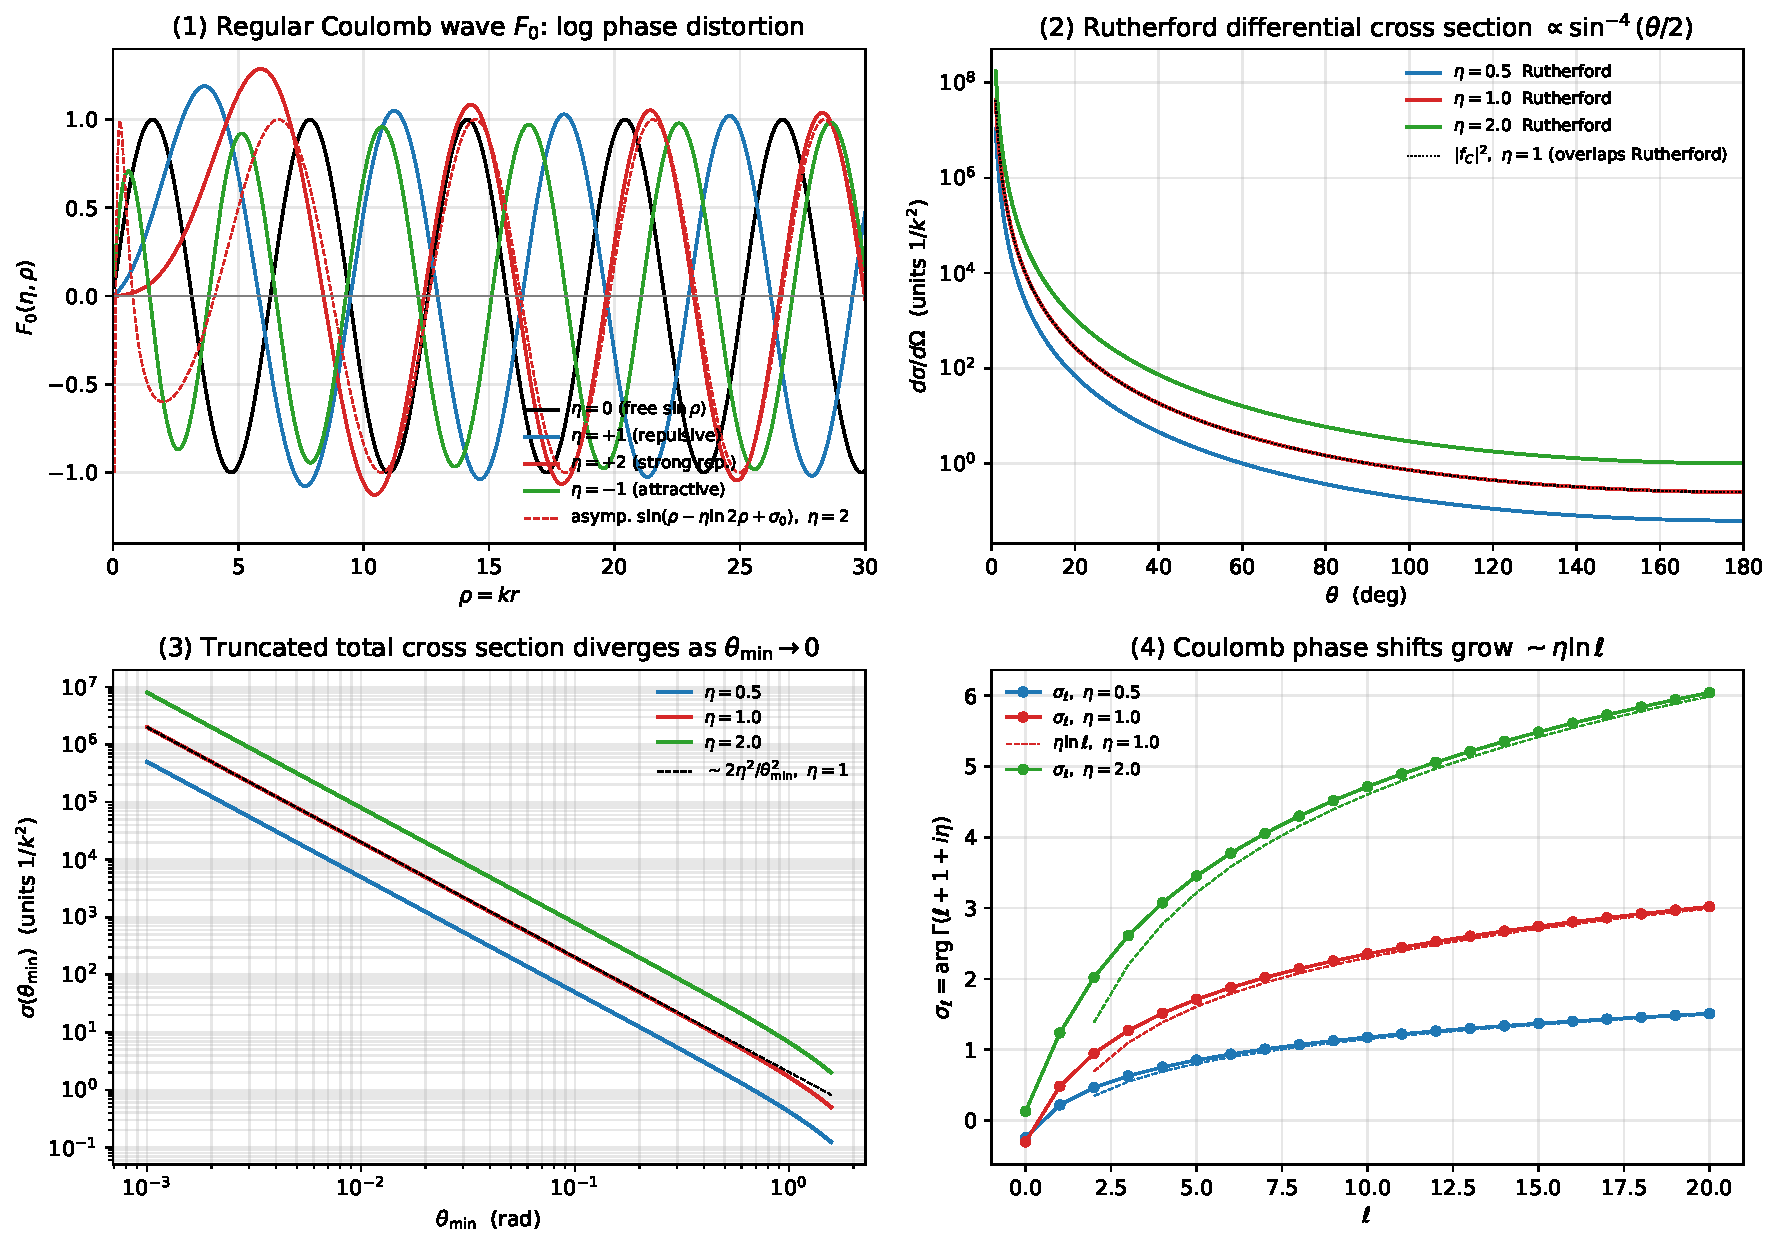
\includegraphics[width=0.95\linewidth]{ch12_coulomb}
    \caption{Coulomb 散射的四组数值验证。
      (1) 正则 Coulomb 函数 $F_0(\eta,\rho)$ 与自由 $\sin\rho$ ($\eta=0$)
      的对比：$\eta>0$ 排斥情形相位在每个周期向外推（节点远离原点），
      $\eta<0$ 吸引情形相位被往内拽；$\eta=2$ 红色虚线即渐近形式
      $\sin(\rho-\eta\ln 2\rho+\sigma_0)$，与精确 $F_0$ 在大 $\rho$ 处吻合。
      (2) 三组 $\eta$ 的 Rutherford 微分截面 $\eta^2/[4k^2\sin^4(\theta/2)]$
      （log 标度）；黑色点线 $|f_C|^2$ 与解析 Rutherford 完全重合，证实
      \eqref{eq:coulomb-fC} 的对数相位不进入 $|\cdot|^2$。
      (3) 截断总截面 $\sigma(\theta_{\min})$ 双对数图，三条线斜率 $-2$，
      与渐近 $4\pi\eta^2/\theta_{\min}^2$（黑色虚线）一致：
      $\theta_{\min}\to 0$ 时 $\sigma\to\infty$，反映 Coulomb 长程性。
      (4) Coulomb 相移 $\sigma_\ell=\arg\Gamma(\ell+1+\rmi\eta)$ 对
      $\eta=0.5,1,2$；虚线 $\eta\ln\ell$ 给出大 $\ell$ 渐近。
      可见所有 $\ell$ 上 $\sigma_\ell\ne 0$ 且不衰减。}
    \label{fig:numexp-ch12}
\end{figure}

\subsection*{物理讨论}

数值结果直接印证了本章三个核心论断。

\paragraph{对数相位畸变是真实的、不可消除的。}
图~\ref{fig:numexp-ch12}(1) 中 $\eta\ne 0$ 的 $F_0$ 与 $\eta=0$ 的
自由解 $\sin\rho$ 在大 $\rho$ 处节点位置渐行渐远 —— 这正是
$-\eta\ln 2\rho$ 项的几何体现：节点条件
$kr-\eta\ln 2kr+\sigma_0=n\pi$ 给出 $r_n\approx (n\pi-\sigma_0+\eta\ln 2kr_n)/k$，
节点间距随 $r$ 缓慢漂移。这种漂移\emph{不能}通过把对数项归入相移来消除
（\S\ref{sec:coulomb-partial} 已论证），因为它依赖 $r$；这就是为什么
``Coulomb 相移''必须把 $-\eta\ln 2kr$ 显式扣除后只取常数部分
$\sigma_\ell$ 来定义。

\paragraph{Rutherford 公式的``奇迹''。}
图~\ref{fig:numexp-ch12}(2) 说明：尽管振幅 $f_C(\theta)$ 带着复杂的
对数相位 $-\rmi\eta\ln\sin^2(\theta/2)$ 与常数 $\rme^{2\rmi\sigma_0}$
（这些相位的存在使 $f_C$ 本身依赖屏蔽方式），但模方 $|f_C|^2$
化简为纯 $\sin^{-4}(\theta/2)$ —— 这是 \S\ref{sec:coulomb-Rutherford}
所指出的``三层级巧合''（经典、Born、精确）的算术验证。换言之：
角分布是 Coulomb 散射唯一干净的可观测量，而振幅本身不是。

\paragraph{总截面发散与长程性。}
图~\ref{fig:numexp-ch12}(3) 的双对数线性行为 $\sigma\sim 1/\theta_{\min}^2$
直接对应于经典 Rutherford $\theta\sim\eta/(kb)$ 给出的关系
$\theta_{\min}\to 0\Leftrightarrow b_{\max}\to\infty$：任意大碰撞参数
$b$ 处粒子仍受偏转，故``有效散射面积''发散。这是 Coulomb 与短程力
最直观的差异：短程势的总截面有限（光学定理给出 $\sigma_{\mathrm{tot}}=
(4\pi/k)\Im f(0)$ 是有限数），而 Coulomb 的 $f_C(0)$ 本身就发散。

\paragraph{$\sigma_\ell$ 不衰减与分波级数发散。}
图~\ref{fig:numexp-ch12}(4) 中 $\sigma_\ell$ 随 $\ell$ 单调增长且
$\sim\eta\ln\ell$，这立刻暗示分波展开
$f_C=(2\rmi k)^{-1}\sum(2\ell+1)(\rme^{2\rmi\sigma_\ell}-1)P_\ell$
中的``因子''$\rme^{2\rmi\sigma_\ell}-1$ 不衰减，故级数
\emph{不绝对收敛}（与短程势分波相移 $\delta_\ell\to 0$ 形成鲜明对比，
那里级数收敛甚至指数快）。这一现象是 \S\ref{sec:coulomb-partial}
``分波展开仅在 Abel 求和意义下重现 $f_C$'' 的根本原因，并预示着
当短程力叠加于 Coulomb 之上时（\eqref{eq:coulomb-fN}），只有
``Coulomb 修正后的剩余相移'' $\delta_\ell^N$ 才会随 $\ell$ 衰减并
给出收敛的 $f_N$。

\paragraph{从数值实验到物理实践。}
本节四张图给出了把 Coulomb 长程性``可视化''的最简方案。在实际数据
分析中（如低能 $p$-$p$、$d$-$\alpha$ 散射），人们观察到的不是裸
Rutherford 而是 \eqref{eq:coulomb-sigma-cross}：Rutherford + 核相移项
+ Coulomb-核子干涉项，干涉项的振荡相位正比于
$\delta_\ell^N-\eta\ln\sin^2(\theta/2)$。本节程序提供的工具
(\texttt{coulomb\_F}, \texttt{sigma\_ell}) 也是分析此类实验数据的基础。

% ===== END CHAPTER =====
